%%%%%%%%%%%%%%%%%%%%%%%%%%%%%%%%%%%%%%%%%
% Thin Sectioned Essay
% LaTeX Template
% Version 1.0 (3/8/13)
%
% This template has been downloaded from:
% http://www.LaTeXTemplates.com
%
% Original Author:
% Nicolas Diaz (nsdiaz@uc.cl) with extensive modifications by:
% Vel (vel@latextemplates.com)
%
% License:
% CC BY-NC-SA 3.0 (http://creativecommons.org/licenses/by-nc-sa/3.0/)
%
%%%%%%%%%%%%%%%%%%%%%%%%%%%%%%%%%%%%%%%%%

%----------------------------------------------------------------------------------------
%	PACKAGES AND OTHER DOCUMENT CONFIGURATIONS
%----------------------------------------------------------------------------------------

\documentclass[a4paper, 11pt]{article} % Font size (can be 10pt, 11pt or 12pt) and paper size (remove a4paper for US letter paper)
\usepackage[polish,british]{babel} % Language support

\usepackage[protrusion=true,expansion=true]{microtype} % Better typography
\usepackage{graphicx} % Required for including pictures
\usepackage{wrapfig} % Allows in-line images

\usepackage{polski}
\usepackage[utf8]{inputenc}
%\usepackage[T1]{fontenc}

% \usepackage{mathpazo} % Use the Palatino font
% \usepackage[T1]{fontenc} % Required for accented characters
% \linespread{1.05} % Change line spacing here, Palatino benefits from a slight increase by default


\makeatletter
\renewcommand{\@listI}{\itemsep=0pt} % Reduce the space between items in the itemize and enumerate environments and the bibliography

\usepackage{url}

\usepackage[font=small]{caption} 
\captionsetup[figure]{}

\renewcommand{\maketitle}{ % Customize the title - do not edit title and author name here, see the TITLE block below
\begin{flushright} % Right align
{\LARGE\@title} % Increase the font size of the title

\vspace{70pt} % Some vertical space between the title and author name

{\large\@author} % Author name
\\\@date % Date

\vspace{40pt} % Some vertical space between the author block aSmith:2013jdnd abstract
\end{flushright}
}

%----------------------------------------------------------------------------------------
%	TITLE
%----------------------------------------------------------------------------------------

\title{\Large \textbf{Creating adjustable cave-like terrain using cellular automata in the context of procedural content generation of strategy game maps} \\ % Title
\large{Project report}} % Subtitle

\author{\textsc{Jakub Sękowski} % Author
\\{\textit{}}} % Institution

\date{\today} % Date

%----------------------------------------------------------------------------------------

\begin{document}

\maketitle % Print the title section

\vspace{60pt}

%----------------------------------------------------------------------------------------
%	ESSAY BODY
%----------------------------------------------------------------------------------------

\section*{Introduction}

\textit{Maps are vital components of level design for many types of games (e.g. first-person shooters, real-time strategy games and flight simulators) and their careful design (manual or procedural) contributes vastly to player experience. There are several reasons [...] why procedural generation of maps is important for game development. First, having an inexhaustible source of new maps means that levels become less predictable, which contributes to the players’ curiosity and the game’s life-span. Second, [...] given that content is represented in an efficient manner and the procedural content generation (PCP) algorithm is parametrizable in the right ways, maps can be adjusted to match player needs and abilities [...]. Finally, PCG can be used as an assisting authoring tool for complementing human creativity and level design expertise existent within commercial game development.} \cite{paper}

In this report, I present the results of studies on automatic terrain generation in a practical setting. I tried to build a framework around cellular automata to create a cave-like terrain shape given realistic constraints. Also, I identified a handful of useful parameters, which can be adjusted in order to control the visual style of the resulting map.

%----------------------------------------------------------------------------------------

\section*{The context}

My work is a part of a project intended to build and maintain a comprehensive map generator for the classic turn-based strategy game Heroes of Might and Magic III \cite{h3}. The project is run by a group of students and employees of University of Wrocław (Institute of Computer Science). The main principles are fairness of the generated maps, sensible and significant logical structure and variety achieved through parameter adjustments as well as random decisions.

The terrain generation is expected to be somewhere in the middle of the process of building the map. The earliest stages are going to produce a logical structure represented as a set of abstract zones and a graph of connections between them. After that, each zone is going to be mapped onto the map grid as a defined chunk of open space. In order to achieve the intended connectivity schema, corresponding to the graph, the zones are going to be surrounded by non-traversable borders except for the precisely positioned walkable cells, acting as portals between selected neighbouring zones. 

Additionally, we have an intention for the terrain to be highly controllable in order to fulfil the typical kinds of requirements in the level design process. Thus, similarly to non-traversable zones' borders, we allow for a cell to be declared as necessarily traversable. The main purpose behind this idea is to be able to set up the paths between the important game facilities, which are guaranteed to remain walkable.

%----------------------------------------------------------------------------------------

\section*{Task specification}

The map is represented as a two-dimensional grid of cells, each of which can be in one of the four feasible states: \emph{black}, \emph{white}, \emph{super-black} or \emph{super-white}. Here is the semantics of these four states:

\begin{itemize}
	\item \emph{white} and \emph{super-white} cells represents traversable terrain;
	\item \emph{black} and \emph{super-black} cells are non-traversable;
	\item cells that are \emph{super-white} and \emph{super-black} are special in a way that their state is immutable; i.e. there is a reason for these cells to be traversable or non-traversable respectively and therefore they must remain such throughout the process.
\end{itemize}

The goal of the terrain generator is to transform the map in such a way that \emph{super} cells remain untouched and the rest is shaped as a reasonably looking strategy game map. More formally:

\begin{itemize}
	\item \textsc{Input:} an arbitrarily filled up grid of cells and a number of parameters, whose possible values and meaning is going to be specified during the process of algorithm design
	\item \textsc{Output:} the new grid that is compatible with the input on the \emph{super-white} and \emph{super-black} cells, and each of remaining ones is either \emph{white} or \emph{black}; it is supposed to respect the input parameters and simultaneously maximise the subjective aesthetic value when interpreted as a cave-like terrain
\end{itemize}

\begin{wrapfigure}{r}{0.0pt}
	\centering
	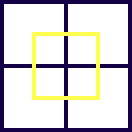
\includegraphics[scale=1.0]{input}
	\caption{Sample map for testing purposes. Dark blue and yellow indicates \emph{super-black} and \emph{super-white} cells respectively. \emph{White} cells are to be changed by the generator.}
	\label{fig:input}
\end{wrapfigure}

As a test case, I am going to use a 33x33 sample input map divided by \emph{super-black} borders into four 15x15 zones. In order to guarantee the connectivity between them throughout the process, middle points of the neighbouring zones are connected with \emph{super-white} line segments through the narrow gaps in the borders (see Figure \ref{fig:input}). The actual inputs are about to be structured similarly except for the possibly more sophisticated shapes of zones and the connectivity schema (not every border is going to have a gap).

%----------------------------------------------------------------------------------------

\section*{Cellular automata}

A cellular automaton is a discrete model developed in the field of artificial life. It consists of (possibly infinite) grid of cells and a fixed rule for changing their states. For each cell there is a set of other cells, defined relative to the specified one (the centre) called its neighbourhood. Typically, the rule of state transition is a mathematical function of a specific cell's current state and its neighbourhood i.e. it depends only on its arguments, it is the same for every cell, it is deterministic and it does not change over time. 

The simulation can be run for an arbitrary initial generation (each cell has some state assigned to it). Then, in each step, the new generation is created by applying the transition rule to every cell in the grid simultaneously.

The two most commonly used types of neighbourhood are the von Neumann neighbourhood and the Moore neighbourhood. The former consists of the four adjacent cells. The latter includes the von Neumann neighbourhood and additionally the four remaining cells surrounding the cell whose state is to be calculated. \cite{wiki} See Figures \ref{fig:moore_neighbourhood} and \ref{fig:neumann_neighbourhood}. A notable well-known example of a cellular automaton is the \emph{Conway's Game of Life} \cite{conway}, whose rule is based on the Moore neighbourhood.

\begin{figure}[ht]
	\centering
	\begin{minipage}[t]{0.45\textwidth}
    		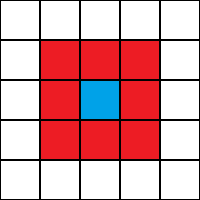
\includegraphics[width=\textwidth]{moore}
		\caption{\textit{The red cells are the Moore neighbourhood for the blue cell.} \cite{wiki}}
		\label{fig:moore_neighbourhood}
	\end{minipage}
	\hfill
	\begin{minipage}[t]{0.45\textwidth}
		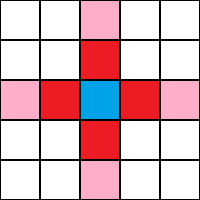
\includegraphics[width=\textwidth]{neumann}
		\caption{\textit{The red cells are the von Neumann neighbourhood for the blue cell. The extended neighbourhood includes the pink cells as well.} \cite{wiki}}
		\label{fig:neumann_neighbourhood}
	\end{minipage}
\end{figure}

A special class of cellular automata is called \emph{outer totalistic cellular automata}. \textit{The state of each cell in a [outer] totalistic cellular automaton is represented by a number (usually an integer value drawn from a finite set), and the value of a cell at time t depends only on the sum of the values of the cells in its neighborhood [...] including the cell itself [...] at time t - 1.} \cite{wiki}

The model I am using in this study is indeed an \emph{outer totalistic cellular automaton}. Cells in states \emph{white} and \emph{super-white} correspond to integer 0. \emph{Black} and \emph{super-black} are seen as 1. The rule is determined by a single number only - a survival threshold. The cell $x$ is \emph{black} in time $t$ if and only if the sum over its neighbourhood in time $t - 1$ is not less then the threshold value, otherwise it is \emph{white}. The rule applies to non-\emph{super} cells only, since \emph{super} states are immutable.

%----------------------------------------------------------------------------------------

\section*{The algorithm}

The generation algorithm works as follows:

\begin{enumerate}
	\item It reads the input map filled with \emph{black}, \emph{white}, \emph{super-black} and \emph{super-white} cells.
	\item Then, to each non-\emph{super} cell, regardless of its current state, it assigns \emph{black} or \emph{white} at random with \textbf{p} being the probability of a \emph{black} state.
	\item It produces the next generation of automaton, by computing the new states for every cell \textbf{x} simultaneously, according to the following rule:
		\begin{itemize}
			\item If \textbf{x} is \emph{super-black} or \emph{super-white}, then its state is preserved in the next generation.
			\item Else,
				\begin{itemize}
					\item let $value(\textbf{y})$ be 1 if cell \textbf{y} is \emph{black} or \emph{super-black} and 0 if it is \emph{white} or \emph{super-white} for every cell \textbf{y};
					\item let \textbf{V} be the sum of cell values over the neighbourhood of \textbf{x};
					\item new state of \textbf{x} is \emph{black} if $\textbf{V} + \textbf{s} \times value(x) \geq \textbf{t}$ and \emph{white} otherwise.
				\end{itemize}
		\end{itemize}
	\item Previous step is repeated until \textbf{i} iterations is reached.
	\item The \textbf{i}-th generation of automaton is returned as a result.
\end{enumerate}

It is easy to see, that this procedure depends on a handful of parameters:

\begin{itemize}
	\item \textbf{p} - the probability of \emph{black} cell in the initial generation of automaton;
	\item \textbf{N} - the neighbourhood type (e.g. Moore, von Neumann);
	\item \textbf{s} - the "self weight" i.e. the degree with which the current state of a cell contributes to its next state calculation;
	\item \textbf{t} - the "survival threshold" i.e. minimal value of $\textbf{V} + \textbf{s} \times value(x)$  necessary for a cell to become (or remain) \emph{black}\footnote{See the algorithm description for details.};
	\item \textbf{i} - the number of generations of cellular automaton to be computed.
\end{itemize}

For the sake of completeness, the random seed used for determining the cells' states in the initial generation should be considered an additional parameter. A set of parameters defined in this manner guarantees an extremely desirable property: the same collection of parameters' values (including the random seed) provided to the algorithm will cause the same map to be regenerated for a particular input.


%----------------------------------------------------------------------------------------

\section*{Evaluation}

\begin{figure}[ht]
	\centering
	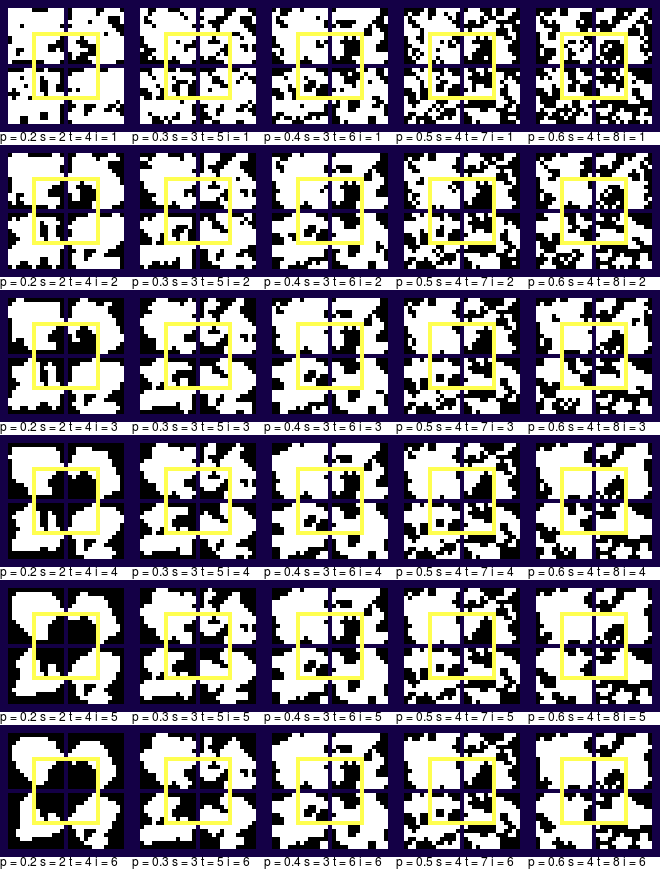
\includegraphics[width=1.\textwidth]{moore_i}
	\caption{Six steps of evolution of the cellular automaton for the Moore neighbourhood and a number of different (\textbf{s}, \textbf{p}) pairs. (\textbf{i} = 1,2,3,4,5,6). Parameter \textbf{t} has been picked automatically.}
	\label{fig:results1}
\end{figure}

\begin{figure}[ht]
	\centering
	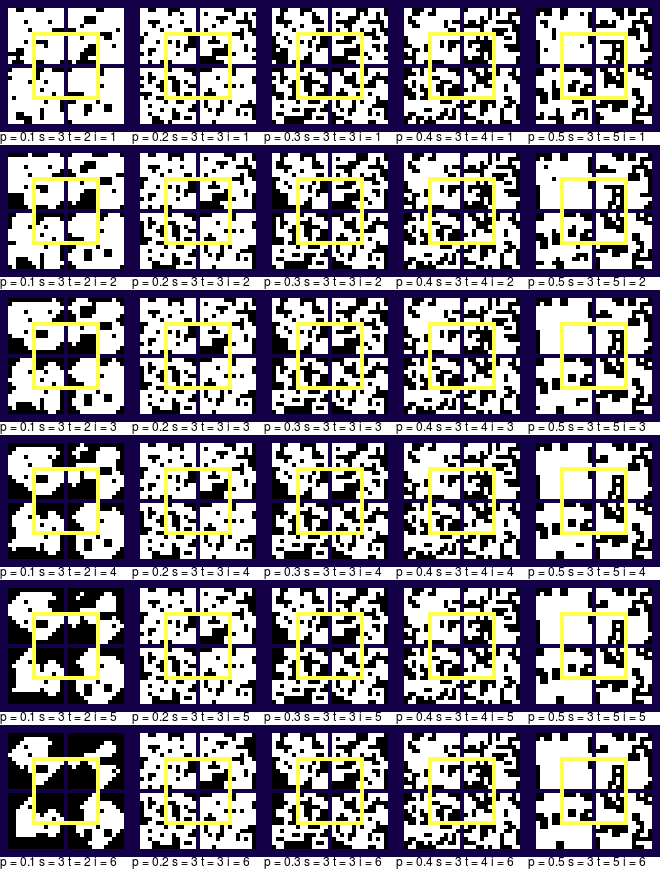
\includegraphics[width=1.\textwidth]{neumann_i}
	\caption{Six steps of evolution of the cellular automaton for the von Neumann neighbourhood and a number of different values of \textbf{p}. (\textbf{s} = 3 \textbf{i} = 1,2,3,4,5,6). Parameter \textbf{t} has been picked automatically.}
	\label{fig:results2}
\end{figure}

\begin{figure}[ht]
	\centering
	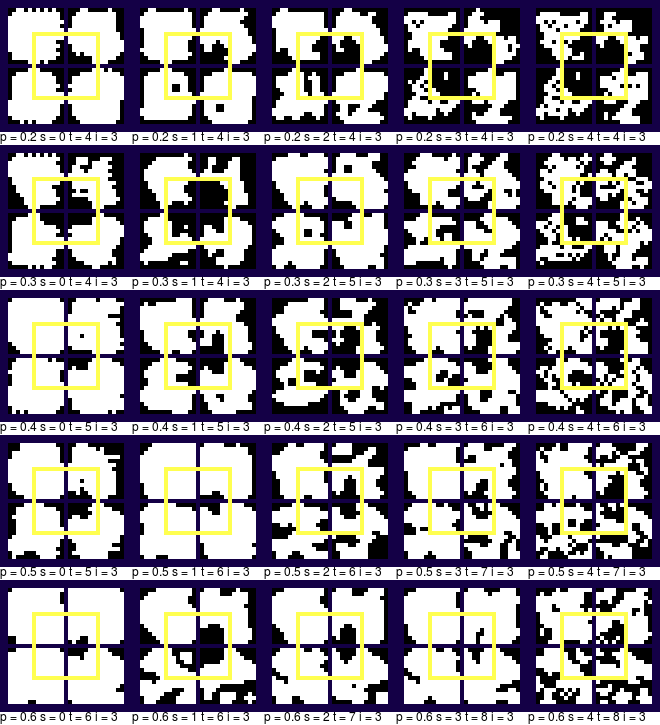
\includegraphics[width=1.\textwidth]{moore_sp}
	\caption{Comparison of results for different values of \textbf{p} and \textbf{s} for Moore neighbourhood and \textbf{i} = 3. Parameter \textbf{t} has been picked automatically.}
	\label{fig:results3}
\end{figure}

\begin{figure}[ht]
        \centering
        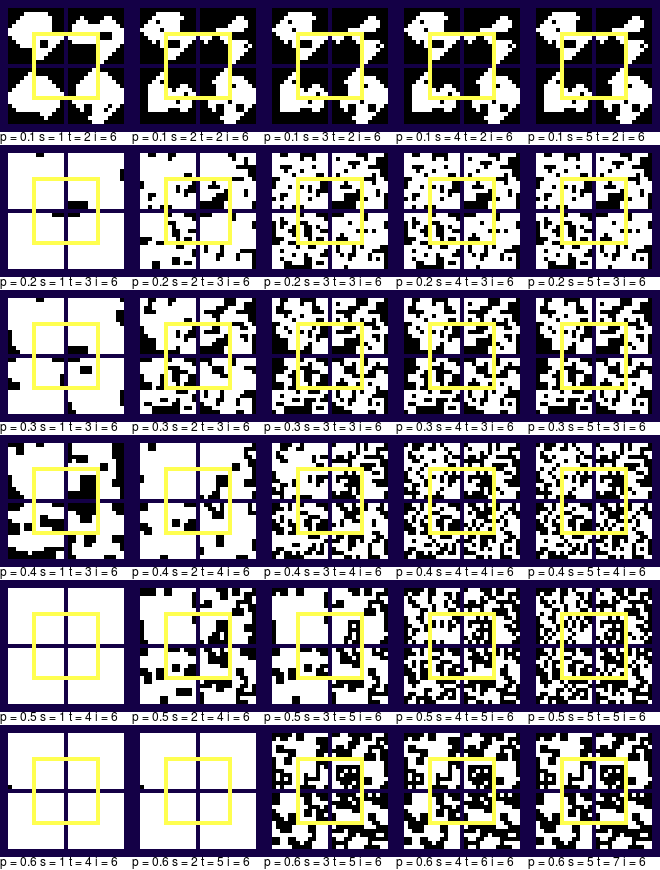
\includegraphics[width=1.\textwidth]{neumann_sp}
	\caption{Comparison of results for different values of \textbf{p} and \textbf{s} for von Neumann neighbourhood and \textbf{i} = 6. Parameter \textbf{t} has been picked automatically.}
	\label{fig:results4}
\end{figure}

I have generated the terrain for the sample input map with a vast variety of the parameters' values. I used both the Moore and von Neumann neighbourhoods. The exact method as well as the parameters are thoroughly described in \emph{The algorithm} section.

In order to highlight the way the parameters affect the result, I reused the initial generations of the automaton as much as possible, since this is the only nondeterministic stage of the procedure. In particular, for each value of parameter \textbf{p} all the generated maps are based upon the same initial state.

Also, I decided to adjust the value of \textbf{t} automatically to suit the selected set of \textbf{p}, \textbf{s} and \textbf{N} values. The reason is that, as preliminary experiments have shown, at most two \textbf{t} values make sense given the other parameters. Usually, a single one can be named that is optimal for generation. Less values lead to maps almost completely filled with \emph{black} cells, whereas greater ones produce maps nearly entirely \emph{white}. In order to pick the right \textbf{t} value I was generating three iterations of automaton for $\textbf{t} = 1,2,3,4...$ and selecting the least \textbf{t} producing the map for which the number of the \emph{white} cells is not less than the number of the \emph{black} cells.

A handful of notable examples of the maps created are presented in Figures \ref{fig:results1}, \ref{fig:results2}, \ref{fig:results3} and \ref{fig:results4}.

Another thing about this way of terrain generation is that the cellular automata are extremely efficient. Computing 6 iterations on 128x128 map using the von Neumann neighbourhood takes only 0.09s on 1.86 GHz CPU. The fact is worth mentioning since it makes the method suitable for real-time generation. 

%----------------------------------------------------------------------------------------

\section*{Conclusion}

As the results show, the cellular automata are the fast and efficient method for generating cave-like terrain on a typical strategy game maps. They can be controlled easily through the convenient notion of immutable cells, which are guaranteed to remain (non)-traversable. The rest of the terrain produced fits these constraints quite naturally. However, earning the specific visual "style" of the map requires careful adjustments of the parameters.

Below, I present the observations I was able to make about each of the parameters, which should be helpful in the process of tweaking and adjusting.

\begin{itemize}
        \item \textbf{N} (the neighbourhood type) is probably the most important parameter. Picking the Moore neighbourhood results in smoothly shaped cave-like structures, which can be seen in Figures \ref{fig:results1} and \ref{fig:results3}. Whereas, the von Neumann neighbourhood produces more right angles and thus the terrain generated resembles more of a labyrinth or a complex of peculiar buildings (see Figures \ref{fig:results2} and \ref{fig:results4}). It looks like some kind of a man-made object. 
	\item In fact, nearly all of the values for parameter \textbf{p} can be used successfully. The near-edge ones, can produce slightly more unexpected results, but not necessarily unwanted.
	\item \textbf{s} affects the "frequency" of a structure. As its value increases the caves' walls become less smooth, there are more rooms disconnected from the main area and the accidental obstacles start to emerge in the middle of the open space. It is well shown in Figure \ref{fig:results3}. The von Neumann neighbourhood works better with slightly greater values of \textbf{s} than the Moore neighbourhood would prefer.
	\item Using the large values of \textbf{i} in most cases is not necessary, since the automaton gets to the "stable" state quickly (see Figures \ref{fig:results1} and \ref{fig:results2}). For this study \textbf{i} = 6 was the maximum, but often 2 or 3 iterations were sufficient.
        \item Parameter \textbf{t} is not really an adjustment, since given the remaining ones, its suitable value may be easily computed. Making this procedure an automatic step is highly recommended, since it decreases the search space substantially.
\end{itemize}

%----------------------------------------------------------------------------------------
%	BIBLIOGRAPHY
%----------------------------------------------------------------------------------------

\bibliographystyle{unsrt}

\begin{thebibliography}{9}
	
\bibitem{h3}
	New World Computing.
	\emph{Heroes of Might and Magic III}.
	The 3DO Company,
	1999.

\bibitem{paper}
	Lawrence Johnson, Georgios N. Yannakakis, and Julian Togelius.
	\emph{Cellular automata for real-time generation of infinite cave levels}.
	\emph{(PCGames '10)}, ACM.
	\url{DOI=http://dx.doi.org/10.1145/1814256.1814266}.

\bibitem{wiki}
        Wikipedia: \emph{Cellular automaton}.
        \url{https://en.wikipedia.org/wiki/Cellular_automaton}.
        Version from 2017-01-05.

\bibitem{conway}
	Wikipedia: \emph{Conway's Game of Life}.
	\url{https://en.wikipedia.org/wiki/Conway's_Game_of_Life}.
	Version from 2017-01-10

\end{thebibliography}

%----------------------------------------------------------------------------------------

\end{document}
